\documentclass[11pt]{article}

\usepackage{latexsym}
\usepackage{algorithm,algpseudocode}
\usepackage{amsmath}
\usepackage{amssymb}
\usepackage{amsthm}
\usepackage{graphicx}
\usepackage{wrapfig}
\usepackage{pseudocode}
\usepackage{subfigure}
\usepackage{url}
\usepackage[backref, colorlinks=true, citecolor=red, urlcolor=blue, pdfauthor={Jyh-Ming Lien}]{hyperref}


\newcommand{\handout}[5]{
  \noindent
  \begin{center}
  \framebox{
    \vbox{
      \hbox to 5.78in { {\bf } \hfill #2 }
      \vspace{4mm}
      \hbox to 5.78in { {\Large \hfill #5  \hfill} }
      \vspace{2mm}
      \hbox to 5.78in { {\em #3 \hfill #4} }
    }
  }
  \end{center}
  \vspace*{4mm}
}

\newcommand{\lecture}[4]{\handout{#1}{#2}{#3}{#4}{#1}}

\newtheorem{theorem}{Theorem}
\newtheorem{corollary}[theorem]{Corollary}
\newtheorem{lemma}[theorem]{Lemma}
\newtheorem{observation}[theorem]{Observation}
\newtheorem{proposition}[theorem]{Proposition}
\newtheorem{definition}[theorem]{Definition}
\newtheorem{claim}[theorem]{Claim}
\newtheorem{fact}[theorem]{Fact}
\newtheorem{assumption}[theorem]{Assumption}

% 1-inch margins, from fullpage.sty by H.Partl, Version 2, Dec. 15, 1988.
\topmargin 0pt
\advance \topmargin by -\headheight
\advance \topmargin by -\headsep
\textheight 8.9in
\oddsidemargin 0pt
\evensidemargin \oddsidemargin
\marginparwidth 0.5in
\textwidth 6.5in

\parindent 0in
\parskip 1.5ex
%\renewcommand{\baselinestretch}{1.25}

\begin{document}

\lecture{Midterm Exam Report}{Fall 2015}{Yeojin Kim}{Advance Algorithm Programming}

\section{Summary of the two methods}

\subsection{hedcuter method}
Hedcuter method consists of two main steps which is slightly different version from Secord's method\cite{secord02}:
\begin{enumerate}
\item Sample initial points $X=\{\mathbf{x_1, x_2, x_3, \cdots}\}$
\item Loop while the displacements don't exceed maximum site displacement and the number of iterations doesn't exceed maximum number of iterations,
\begin{enumerate}
\item Map the image value at $\mathbf{x_i}$ to stipple level $t$
\item Propagate the stipple level at $\mathbf{x_i}$ to its neighbor  
\item Compute the centroids%%%%% copy stipples?
\item Move each points $\mathbf{x_i}$ to its new centers of a cell $\mathbf{C_i}$
\end{enumerate}
\end{enumerate}
%%%%% author's idea?
%%%%%Sampling
Sampling\\\\
%2. Loop
In the loop, the algorithm keeps mapping image using the location of a point(which corresponds to the coordinates of a pixel) as unique identification. This mapping image contains stipple level $t$ at each points with the number of levels $l$. 
Unlike Secord's method\cite{secord02}, hedcuter method first computes and stores stipple level $t$ only at given points using Eq. \ref{eq:distance}. Next, it sort the stipples with stipple level, $x$ values, and $y$ values. 
\begin{equation}\label{eq:distance}
t=\frac{l-I(\mathbf{x})*\rho(\mathbf{x})}{l},\:\:where\:\:\rho(\mathbf{x})=1\:\:\forall x %%%%% More details about Intensity?
\end{equation}

After propagation, hedcuter method collect pixels covered with a voronoi cell. 

\subsection{voronoi method}
A flow of voronoi method basically follows Lloyd's method\cite{Okabe:1992:STC:135734}, which as follows : \\ 
when the centroid of a region is defined as
\begin{equation}\label{eq:centroid}
\mathbf{C_i}=\frac{\int_{A}\mathbf{x}\rho(\mathbf{x})dA}{\int_{A}\rho(\mathbf{x})dA},
\end{equation}
\begin{algorithm}
\caption{Lloyd's method}\label{alg:lloyds}
\begin{algorithmic}[1]
\While {generating point $\mathbf{x_i}$ not converged to centroids}
    \State Compute the Voronoi diagram of $\mathbf{x_i}$
    \State Compute the centroids $\mathbf{C_i}$ using equation (\ref{eq:centroid})
    \State Move each generating point $\mathbf{x_i}$ to its centroids $\mathbf{C_i}$
\EndWhile
\end{algorithmic}
\end{algorithm}\\
For more simple explanation of details, let's assume that we have a part of image(Fig. \ref{fig:intensity}) from squirrel's back. %%%%%ref here
First, voronoi method samples points on the image randomly(Fig. \ref{fig:samples}). %%%%%check uniform random or gaussian random
\begin{figure*}[hbt]
 \centering
 \subfigure[]{
    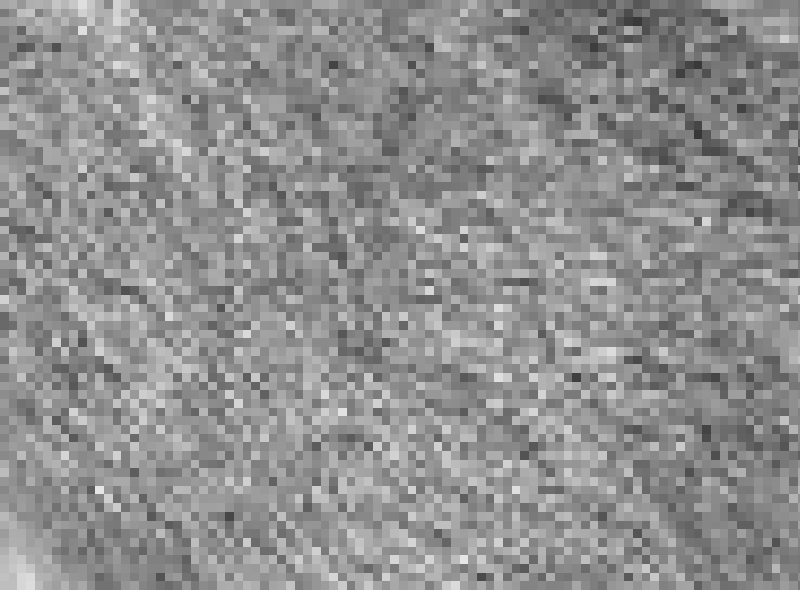
\includegraphics[width=0.32\textwidth]{FIGS/intensity.png}
    \label{fig:intensity}
  }\hspace{-3mm}
  \subfigure[]{
    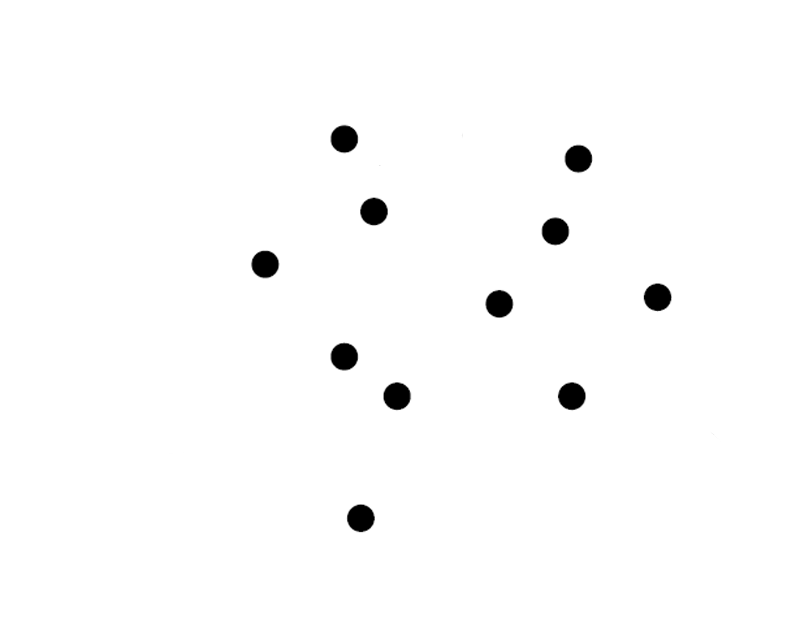
\includegraphics[width=0.32\textwidth]{FIGS/sites.png}
    \label{fig:samples}
  }\hspace{-3mm}
    \caption{A part of given image and sample points. \label{fig:sampling}}
\end{figure*}\\
\begin{figure*}[thb]
 \centering
 \subfigure[]{
    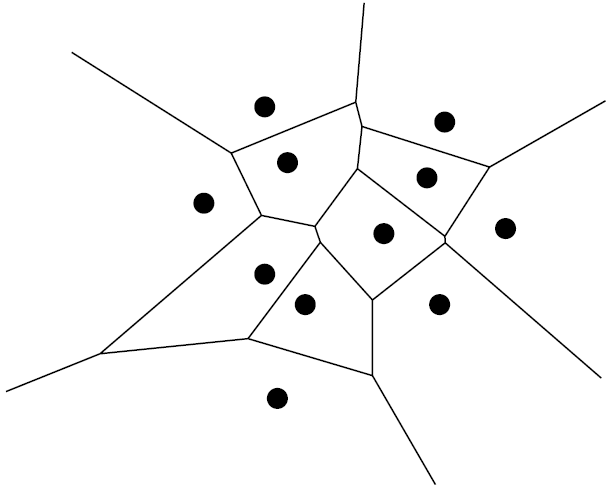
\includegraphics[width=0.32\textwidth]{FIGS/voronoi.png}
    \label{fig:voronoi}
  }\hspace{-3mm}
  \subfigure[]{
    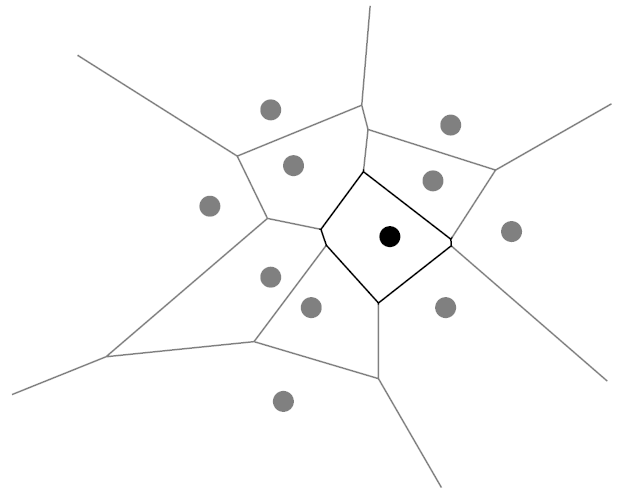
\includegraphics[width=0.32\textwidth]{FIGS/cell.png}
    \label{fig:cell}
  }\hspace{-3mm}
   \subfigure[]{
    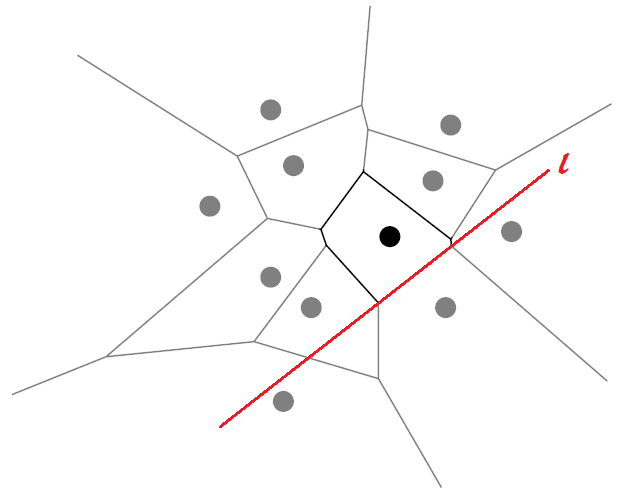
\includegraphics[width=0.32\textwidth]{FIGS/clippedLine.png}
    \label{fig:subpixel}
  }\\
  \subfigure[]{
    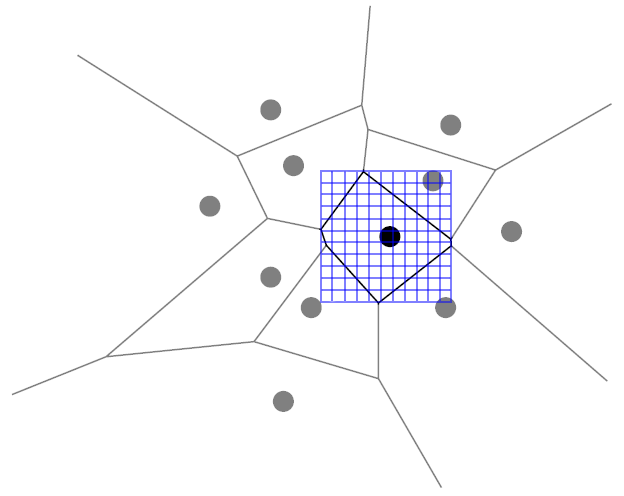
\includegraphics[width=0.32\textwidth]{FIGS/subpixel.png}
    \label{fig:subpixel}
  }\hspace{-3mm}
  \subfigure[]{
    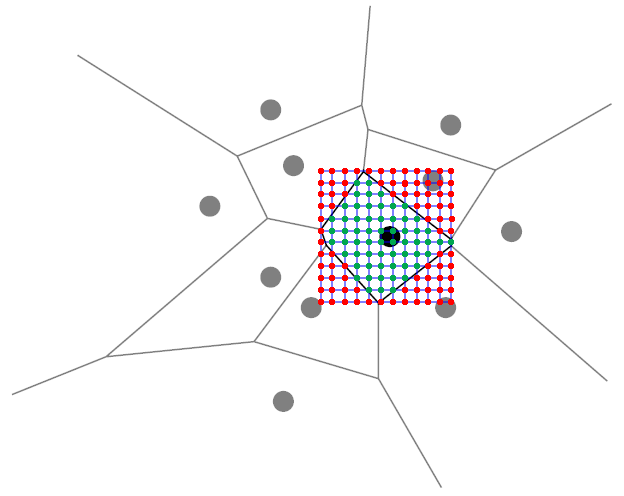
\includegraphics[width=0.32\textwidth]{FIGS/inandout.png}
    \label{fig:inOutTest}
  }\hspace{-3mm}
  \subfigure[]{
    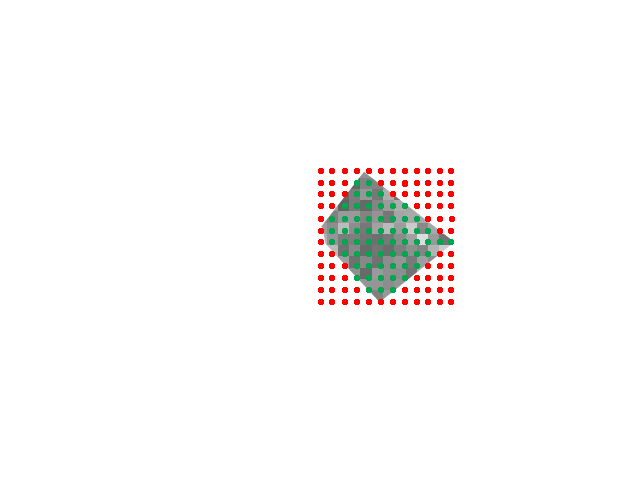
\includegraphics[width=0.32\textwidth]{FIGS/integral.png}
    \label{fig:integral}
  }\hspace{-3mm}
    \caption{The progress of computing voronoi diagram and redistributing stipples. \label{fig:createVoronoi}}
\end{figure*}
Next, voronoi method computes the voronoi region of given sample points(Fig. \ref{fig:voronoi}).
After creating voronoi diagram of given points, the algorithm computes the centroid of a cell iteratively looping through all these points.
For example, with a given cell in Fig. \ref{fig:cell}, voronoi method calculates the line which is the extension of voronoi edge and is called clipping line.
When two end points of voronoi edge are $\mathbf{x_1}=(x_1,y_1)$ and $\mathbf{x_2}=(x_2,y_2)$, the equation of clipping line is
\begin{equation}\label{eq:clippingLine}
\begin{gathered}
(y-y_1) = \frac{(y_2-y_1)}{(x_2-x_1)}(x-x_1)\\
(y-y_1)(x_2-x_1) = (y_2-y_1)(x-x_1)\\
(y_2-y_1)(x-x_1)-(y-y_1)(x_2-x_1)= 0\\
(y_2-y_1)x-(x_2-x_1)y+y_1(x_2-x_1)-x_1(y_2-y_1)=0\\
-(y_1-y_2)x+(x_1-x_2)y+x_1(y_1-y_2)-y_1(x_1-x_2)=0\\\\
\therefore ax+by+c=0 \\where\:a=-(y_1-y_2),\:b=(x_1-x_2),\:and\:c=x_1(y_1-y_2)-y_1(x_1-x_2).
\end{gathered}
\end{equation}
In the same way, we can generate clipping lines for all voronoi edges in a cell.\\\\
To obtain the integration of density $\rho(\mathbf{x})$, voronoi method creates grid on a cell with the user-specified number of subpixels(Fig. \ref{fig:subpixel}).
Using the clipping lines(Eq. \ref{eq:clippingLine}), we can test if a grid point is inside or outside of cell. If a grid point $\mathbf{x_g}=(x_g, y_g)$ satisfies $ax_g+by_g+c<0$ for all the clipping lines, it locates inside of a cell. The result of test is shown in Fig. \ref{fig:inOutTest}. The red points mean outside and the green points mean inside.
\\When grid points are inside, the algorithm obtains $\int_{A}\rho(\mathbf{x})dA$ and $\int_{A}\mathbf{x}\rho(\mathbf{x})dA$ with intensity $I(\mathbf{x_g})$ which has corresponding location to grid points in grayscale image(Fig. \ref{fig:integral}, Eq. \ref{eq:density}).
\begin{equation}\label{eq:density} %%%%% more details about intensity? such as formula? %% gaussian numerical integration, --- from web sites.
\begin{gathered}
\int_{A}\rho(\mathbf{x})dA=\int I(\mathbf{x_g})\\
\int_{A}\mathbf{x}\rho(\mathbf{x})dA=\int \mathbf{x}I(\mathbf{x_g})=\int (x, y)I(\mathbf{x_g}).
\end{gathered}
\end{equation}
Substituting the results of Eq. \ref{eq:density} to Eq. \ref{eq:centroid}, we can generate new centroid $\mathbf{C_i}=(x_c, y_c)$,
which satisfies that $x_c=\frac{\int x\cdot I(\mathbf{x_g})}{\int I(\mathbf{x_g})}$ and $y_c=\frac{\int y\cdot I(\mathbf{x_g})}{\int I(\mathbf{x_g})}$.%%%%% writing about radius?
This new centroids will be fed as sites into creating voronoi diagram step. Voronoi method repeats creating voronoi diagram and computing the centroid repeatedly until the average of displacement between points $\mathbf{x_i}$ and centroids $\mathbf{C_i}$ is small enough.
%%%%% contents about radius?
\section{Comparison of the two methods}

\section{Improvement of hedcuter method}

\bibliographystyle{plain}
\bibliography{report}

\end{document}


